\documentclass[table]{scrreprt}
\setcounter{secnumdepth}{5}
\usepackage{graphicx}
\usepackage[utf8]{inputenc}
\usepackage{tikz}
\usepackage{listings}
\usepackage{underscore}
\usepackage[bookmarks=true]{hyperref}
\usepackage{placeins}
\usepackage{caption}
\usepackage{xcolor}

\hypersetup{
    bookmarks=false,    % show bookmarks bar?
    pdftitle={Software Requirement Specification},    % title
    pdfauthor={},                     % author
    pdfsubject={TeX and LaTeX},                        % subject of the document
    pdfkeywords={TeX, LaTeX, graphics, images}, % list of keywords
    colorlinks=true,       % false: boxed links; true: colored links
    linkcolor=blue,       % color of internal links
    citecolor=black,       % color of links to bibliography
    filecolor=black,        % color of file links
    urlcolor=purple,        % color of external links
    linktoc=page            % only page is linked
}%
\def\myversion{1.0}
\date{}
\usepackage{hyperref}
\begin{document}
    \begin{titlepage}
        \flushright\bfseries\huge
        \vspace*{\stretch{0.4}}
        \rule{\linewidth}{5pt}
        \par
        \vspace{1cm}
        {\Huge MASTER \par TEST \par DOCUMENT \par}
        \vspace{2cm}
        for \\
        \vspace{2cm}
        Personal Dietary Application \\
        \vspace{2cm}
        \LARGE{Version \myversion \\}
        \vspace{2cm}
        by Craig Boucher \\
        Md Tanveer Alamgir \\
        Fan Zou\\
        Osman Momoh \\
        Xin Ma
        \vspace{2cm}
        \rule{\linewidth}{5pt}
        \vspace{\stretch{1}}
    \end{titlepage}

    \tableofcontents

    \chapter{Introduction}
    This master testing document describes the strategies and tools we (Team 4) used to test the Personal Dietary Manager application. This testing document serves as the deliverable document for iteration 3 of the class project in COMP 5541 at Concordia Univeristy. Iteration 3 is the final iteration of of Personal Dietary Manager, and implements database functionality using MySQL. \\ \\
    Associated with this test plan are documents delivered in iteration 1 and iteration 2 of this project. These are, respectively, the Software Requirements Specifications (SRS) and Design Documents (DD). This test plan will refer to these other documents for the purpose of traceability.

    \section{Purpose}
    The purpose of this test plan is to verify the quality and correctness of the Personal Dietary Manager application. Correctness is the state in which the application satisfies the SRS and delivers a product that can accurately track a dietary regimen. Quality is the state in which the application delivers a user-friendly experience that is free of bugs, runs fast, and runs smoothly. \\\\
    As no software project is perfect, any outstanding bugs and issues will also be discussed.

    \section{Scope}
    The scope of this test document are the tools are strategies that are used for testing. These are:
    \begin{itemize}
        \item Unit testing
        \item Integration and Module Testing
        \item Functional Testing
        \item User Interface Testing
    \end{itemize}
    Tests that are outside of the scope of this document are load, configuration and installation, business analysis, network security, and stress testing.


    \section{Document Terminology and Acronyms}

    \begin{tabular}{|l|l|}
        \hline
        \textbf{Abbreviation} & \textbf{Term} \\
        \hline
        MVC & Model View Controller \\
        \hline
        GUI & Graphical User Interface \\
        \hline
        UML & Unified Modeling Language \\
        \hline
        PDA & Personal Dietary Application \\
        \hline
        GRASP & General Responsibility Assignment Software Patterns \\
        \hline
    \end{tabular}

    \section{References}

    \begin{itemize}

        \item Dr. Nora Houari, 2020, ``COMP 5541 Course Notes" including:
        \begin{itemize}
            \item Introduction to testing
            \item Tutorial: Testing
            \item Project Information
            \item Montrealopoly Master Test Plan
        \end{itemize}
        \item Pressman, R.S. (2009). Software Engineering: A Practitioner's Approach, 7Th Edition.

        \item ISO/IEC/IEEE International Standard - Software and systems engineering -- Software testing --Part 3: Test documentation," in ISO/IEC/IEEE 29119-3:2013(E) , vol., no., pp.1-138, 1 Sept. 2013

    \end{itemize}

    \chapter{Evaluation Mission Test Motivation}
    
    The purpose of this test document is to ensure the personal dietary desktop application meets the design requirements mandated by the course objectives outlined in the project specification document and system requirements document. This document will be a tool to outline test cases and keep a quality assurance guideline for the software development team. Lastly, the 'team 4' group will deliver an exceptional piece of quality software.

    \section{Background}
The graduate diploma course COMP 5541 mandated a personal dietary application be developed as part of a group project for the semester. The third increment of this project involved implementing a database for use with the desktop application. A remote database server offered by Microsoft, Azure, is utilized. The Java programming language and GUI library JavaFX. A comprehensive testing environment has been created to make sure the software is completed without any major issues or bugs. 
\par
This test document outlines several testing methods and processes that were used to verify the software is without serious bugs. The previous document included, the design document, had the software architecture and design pattern specifications. The initial document, the requirements document, contained the class diagrams, use case diagrams, and the purpose and demands the software is intended to fulfill.

    \section{Evaluation Mission}
    The principal goals of this document are evaluated as the following:
    \begin{itemize}
    \item Making sure that the design document quality is adhered to.
    \item Guaranteeing the software requirement document specifications are completed.
    \item That any major software bugs are not found in the application.
    \end{itemize}
    
    The test plan document will be used as a tool to make sure these missions are accomplished.
    
\newpage 

    \section{Test Motivators}
    The areas explored in this testing document are the following:
\\    \\
    \textbf{Unit Testing}: A set number of methods are tested to verify their inputs and outputs meet the specifications. White and black box testing methods are used.\\
    \textbf{Integration and Module Testing}: The classes and objects are tested together to see if behavior remains consistent. \\
    \textbf{Functional Testing}: Makes sure that use cases objectives are accomplished.
    \newline
    \textbf{User Interface Testing}: The GUI that the user interacts with is checked for malfunctions. 
    
    \chapter{Outline of Planned Tests}

    This section provides an overview of the four types of tests that we will do: unit testing, integration and module testing, functional testing, and user interface testing. A brief description of each is described. \\ \\
    We frequently distinguish our testing strategies between white- and black-box testing. White-box testing tests the internal structures of an application (e.g. source code, classes, methods). Conversely, black-box testing tests the external functions that the software is supposed to perform, and does not necessarily examine the underlying source code.

    \section{Unit Testing}
    The primary focus of unit testing is performing isolated tests on specific methods in the system. We we will be using white box testing techniques to iterate through the paths the methods take to execute their instructions. The following list of methods is not every method present in the software application however they are the most crucial. For a complete list of the methods please see the design document. Here are the methods included in this document which are tested: \\
    \begin{itemize}
    \item Method createDining
    \item Method deleteDining
    \item Method findDiningByName
    \item Method createMeal
    \item Method createRetailer
    \end{itemize}

    \section{Integration and Module Testing}
    
    The integration and module testing will verify that the classes and methods work together as a larger system. There is only one main window for the personal dietary application. Both bottom up and top down testing are used when describing the test cases and their results for the functionality available to the user in the main window. From the main window, every piece of the model view controller (MVC) model is coordinated to deliver the appropriate software functionality.

    \section{Functional Testing}
    Functional testing is a form a black-box testing in which the application use cases are tested. These use cases can be found both in the SRS and the Project Infromation class notes document. In other words, the functional requirements of the project are tested for correctness.

    \section{User Interface Testing}
    User interface (UI) testing involves testing the various parts of the GUI for correctness and quality. These GUI parts include the text fields, comboboxes, observable lists, list views, table views, buttons, etc. UI testing is a form of black-box testing.

    \chapter{Test Approach}

    \section{Unit Testing}
    Individual methods are tested here, in the unit testing portion of the testing phase. The methods have been integrated to perform with the latest increment of the development for this personal dietary application. Therefore, they have database functionality.

    \subsection{createDiningTest()}
    The createDining() method initialized a Dining item to be added to an observable list. This list keeps track of all the dining items input by the user. The Dining items are also added to the database.
    \begin{verbatim}
public void createDiningTest() throws SQLException {
        DiningDAO diningDAO= new DiningDAOImp();
        FoodGroup foodGroup=new FoodGroup("vegetables_and_fruits");
        foodGroup.setFoodGroupId(1);
        Meal meal=new Meal("coffee");
        meal.setMealId(3);
        Type type=new Type("homemade");
        type.setTypeId(1);
        Retailer retailer=new Retailer("McDonald");
        retailer.setRetailerId(4);
        Serving serving = new Serving("1 cup", 10, 10, 10, 10);

        Indining indining=new Indining();
        indining.setName("testIndining");
        indining.setConsumed(false);
        indining.setFoodGroup(foodGroup);
        indining.setMeal(meal);
        indining.setTime(LocalDateTime.now());
        indining.setType(type);
        indining.setServing(serving);

        int inResult = diningDAO.createDining(indining);
        Dining inFound= diningDAO.findDiningById(indining.getDiningId());

        Serving serving2 = new Serving("1 cup", 20, 20, 20, 20);
        Outdining outdining=new Outdining();
        outdining.setName("testOutdining");
        outdining.setConsumed(false);
        outdining.setFoodGroup(foodGroup);
        outdining.setMeal(meal);
        outdining.setTime(LocalDateTime.now());
        outdining.setRetailer(retailer);
        outdining.setServing(serving2);
        int outResult = diningDAO.createDining(outdining);
        Dining outFound= diningDAO.findDiningById(outdining.getDiningId());

        assertEquals("T0---Create Dining", 1, inResult);
        assertEquals("T0---createInDiningTest", inFound, indining);
    }

\end{verbatim}

Unit test case passes.


\subsection{deleteKnownDiningTest()}
The delete method removes the dining item from the list and from the database.

\begin{verbatim}
    public void deleteKnownDiningTest() throws SQLException {
        DiningDAO diningDAO= new DiningDAOImp();
        int result = diningDAO.deleteDining(31);
        assertEquals("T30---deleteKnownDiningTest: ", 1, result);
    }
\end{verbatim}

Unit test case passes.

\subsection{findFoodGroupByNameTest()}
Every food item has an associated food group. This method will find the food group that has been associated to the food item.

\begin{verbatim}
    public void findFoodGroupByNameTest() throws SQLException {
        FoodGroupDAO foodGroupDAO= new FoodGroupDAOImp();
        String name="grain_products";
        FoodGroup foodGroup =foodGroupDAO.findFoodGroupByName(name);
        assertEquals("T3---findFoodGroupByName: ", name, foodGroup.getFoodGroupName());
    }
\end{verbatim}

Unit test case passes.

\subsection{createMealTest()}

The createMeal() method instantiates the necessary meal object to be used in the software application. The data given by the user indicates what kind of meal object to create with dedicated attributes.

\begin{verbatim}
   public void createMealTest() throws SQLException {
        MealDAO mealDAO= new MealDAOImp();
        Meal meal1=new Meal(), meal2 = new Meal();
        meal1.setMealName("test7");
        meal2.setMealName("test8");

        int result = mealDAO.createMeal(meal1);
        int result2 = mealDAO.createMeal(meal2);
        Meal found= mealDAO.findMealById(meal1.getMealId());
        Meal found2 = mealDAO.findMealById(meal2.getMealId());
        assertEquals("T0---Create Meal", 1, result);
        assertEquals("T0---Create Meal", 1, result2);
        assertEquals("T0---CreateMealTest", found, meal1);
        assertEquals("T0---CreateMealTest", found2, meal2);
    }
\end{verbatim}

Unit test case passes.

\subsection{createRetailerTest()}

For an out dining object, the createRetailer() method will instantiate the necessary retailer object. The data is fed to the database as necessary.

\begin{verbatim}
    public void createRetailerTest() throws SQLException {
        RetailerDAO retailerDAO= new RetailerDAOImp();
        Retailer retailer=new Retailer();
        retailer.setRetailerName("test3");

        int result = retailerDAO.createRetailer(retailer);
        Retailer found= retailerDAO.findRetailerById(retailer.getRetailerId());
        assertEquals("T0---Create retailer", 1, result);
        assertEquals("T0---CreateRetailerTest", found, retailer);
    }
\end{verbatim}

Unit test case passes.

\newpage

    \section{Integration and Module Testing}
    The integration and module testing observes, tests, and sees how different parts of the application operate together. \par
    The personal dietary application has several modules that work together to form a Model-View-Controller (MVC) architecture. There is only one window, the main window, from which all operations can be performed. Several test cases were reviewed to ensure the overall architecture of the application is well integrated and working properly.
    % Explain the MVC work together and the database... leads to the test cases.

    \subsection{Main Window}
    
    \newcolumntype{a}{>{\columncolor{yellow}}c}	

	\def\arraystretch{1.5}
		\begin{tabular}{|a|p{12cm}|}
	\hline
		\textbf{Test Case 1} &  Application opens to main window \\
	\hline
		 \textbf{Test Case Description} & Test to see if the main window opens. This test case is performed when the program is run. \\ 
	\hline
		\textbf{Result} & Passed \\
	\hline
	\end{tabular}
	\\ \\ \\
		\def\arraystretch{1.5}
		\begin{tabular}{|a|p{12cm}|}
	\hline
		\textbf{Test Case 2} &  Data is read from text boxes \\
	\hline
		 \textbf{Test Case Description} & When the application is launched with the main window visible, test to see if the text boxes on the left hand side can read input. \\ 
	\hline
		\textbf{Result} & Passed \\
	\hline
	\end{tabular}
		\\ \\ \\
		\def\arraystretch{1.5}
		\begin{tabular}{|a|p{12cm}|}
	\hline
		\textbf{Test Case 3} &  Events are handled by controller \\
	\hline
		 \textbf{Test Case Description} & Several events are initiated by the various buttons the user can interact with in the main window. Attempt to test them by using their operations. \\ 
	\hline
		\textbf{Result} & Passed \\
	\hline
	\end{tabular}
    	\\ \\ \\
		\def\arraystretch{1.5}
		\begin{tabular}{|a|p{12cm}|}
	\hline
		\textbf{Test Case 4} & Information is saved to database \\
	\hline
		 \textbf{Test Case Description} & The items recorded by the application are transferred from main memory to the database. Tested by adding items with the provided buttons. \\ 
	\hline
		\textbf{Result} & Passed \\
	\hline
	\end{tabular}
		\\ \\ \\
		\def\arraystretch{1.5}
		\begin{tabular}{|a|p{12cm}|}
	\hline
		\textbf{Test Case 5} &  Necessary data is loaded from database \\
	\hline
		 \textbf{Test Case Description} & After saving data in the system, close the application and relaunch the application to observe if data is still present. \\ 
	\hline
		\textbf{Result} & Passed \\
	\hline
	\end{tabular}

    \section{Functional Testing}

	In this section we outline the tests done for the functional requirements (a.k.a use cases). A list of these use cases can be found in the SRS and Project 			Information class notes.
	
	\subsection{}
	
	\newcolumntype{a}{>{\columncolor{green}}c}	

	\def\arraystretch{1.5}
		\begin{tabular}{|a|p{13cm}|}
	\hline
		\textbf{Use Case} &  View a list of all foods in diet \\
	\hline
		 \textbf{Description} & The user is able to view a list of foods (both consumed and not consumed) \\ 
	\hline
		\textbf{Preconditions} & The user has entered food items into list \\
	\hline
		\textbf{Postconditions} & A list of foods is displayed on the center portion of the application \\
	\hline
		\textbf{Comments} & Test sucessful \\
	\hline
	\end{tabular}

	\subsection{}
	\def\arraystretch{1.5}
		\begin{tabular}{|a|p{13cm}|}
	\hline
		\textbf{Use Case} &  Add a new food item\\
	\hline
		 \textbf{Description} & A new food item is added to the list of foods \\ 
	\hline
		\textbf{Preconditions} & The user has inputted all text fields with appropriate data \\
	\hline
		\textbf{Postconditions} & A new food item appears at the end of the displayed food list \\
	\hline
		\textbf{Comments} & Test sucessful \\
	\hline
	\end{tabular}

	\subsection{}
	\def\arraystretch{1.5}
		\begin{tabular}{|a|p{13cm}|}
	\hline
		\textbf{Use Case} &  Mark a food group as eaten or not eaten \\
	\hline
		 \textbf{Description} & A food group will be marked as eaten if a food item is consumed of that group. It will be marked not eaten if there are no consumed food items in that group \\ 
	\hline
		\textbf{Preconditions} &  The presence, or not, of food items in the food list \\
	\hline
		\textbf{Postconditions} & The appropriate food group box will light up at the bottom of the application \\
	\hline
		\textbf{Comments} & Test sucessful \\
	\hline
	\end{tabular}

	\subsection{}
	\def\arraystretch{1.5}
		\begin{tabular}{|a|p{13cm}|}
	\hline
		\textbf{Use Case} &  Mark a food group as eaten or not eaten \\
	\hline
		 \textbf{Description} & A food group will be marked as eaten if a food item is consumed of that group. It will be marked not eaten if there are no consumed food items in that group \\ 
	\hline
		\textbf{Preconditions} &  The presence, or not, of food items in the food list \\
	\hline
		\textbf{Postconditions} & The appropriate food group box will light up at the bottom of the application \\
	\hline
		\textbf{Comments} & Test sucessful \\
	\hline
	\end{tabular}

	\subsection{}
	\def\arraystretch{1.5}
		\begin{tabular}{|a|p{13cm}|}
	\hline
		\textbf{Use Case} &  Remove a food item \\
	\hline
		 \textbf{Description} & A food item in the food list is removed \\ 
	\hline
		\textbf{Preconditions} & One or more food items are in the food list \\
	\hline
		\textbf{Postconditions} & The selected food item is removed from the food list \\
	\hline
		\textbf{Comments} & Test sucessful \\
	\hline
	\end{tabular}

	\subsection{}
	\def\arraystretch{1.5}
		\begin{tabular}{|a|p{13cm}|}
	\hline
		\textbf{Use Case} & Sort the food list based on a food attribute (e.g. serving, time, food group) \\
	\hline
		 \textbf{Description} & The list of foods is sorted based on a given food attribute \\ 
	\hline
		\textbf{Preconditions} & Two or more food items are in the food list \\
	\hline
		\textbf{Postconditions} & The foods in the food list are sorted in ascending or descending order based on the attribute \\
	\hline
		\textbf{Comments} & Test sucessful \\
	\hline
	\end{tabular}

	\subsection{}
	\def\arraystretch{1.5}
		\begin{tabular}{|a|p{13cm}|}
	\hline
		\textbf{Use Case} & Set a food item as consumed or not consumed \\
	\hline
		 \textbf{Description} & The user is able to select in the list of foods which ones are consumed or not consumed \\ 
	\hline
		\textbf{Preconditions} &  One or more food items are in the food list\\
	\hline
		\textbf{Postconditions} & A food item is marked as consumed or not consumed. The total nutrients in the consumed food list is appropriately updated. \\
	\hline
		\textbf{Comments} & Test sucessful \\
	\hline
	\end{tabular}

	\subsection{}
	\def\arraystretch{1.5}
		\begin{tabular}{|a|p{13cm}|}
	\hline
		\textbf{Use Case} & Choose a food item as either indining or outdining \\
	\hline
		 \textbf{Description} & The user is able to select if the food item has either an indining or outdining food attribute \\ 
	\hline
		\textbf{Preconditions} & The user has entered corrected all values in the text areas \\
	\hline
		\textbf{Postconditions} & A food item is entered into the food list with either an indining or outdining food attribute \\
	\hline
		\textbf{Comments} & Test sucessful \\
	\hline
	\end{tabular}

	\subsection{}
	\def\arraystretch{1.5}
		\begin{tabular}{|a|p{13cm}|}
	\hline
		\textbf{Use Case} & View only consumed food items, or view all food items \\
	\hline
		 \textbf{Description} & The user is able to view either consumed food items, or a list of all food items (consumed and not consumed) \\ 
	\hline
		\textbf{Preconditions} &  Two or more food items are in the food list \\
	\hline
		\textbf{Postconditions} & Either all food items will  be displayed, or only consumed food items \\
	\hline
		\textbf{Comments} & Test sucessful \\
	\hline
	\end{tabular}

	\subsection{}
	\def\arraystretch{1.5}
		\begin{tabular}{|a|p{13cm}|}
	\hline
		\textbf{Use Case} & The food list will persist after application closes \\
	\hline
		 \textbf{Description} & The food list is automatically saved in a database after a food item is added or deleted. The food list is restored upon opening the application \\ 
	\hline
		\textbf{Preconditions} &  The user has previously added or removed food items \\
	\hline
		\textbf{Postconditions} & The food list which existed before closing the application is restored upon opening the application. \\
	\hline
		\textbf{Comments} & Test sucessful \\
	\hline
	\end{tabular}
	\newpage
    \section{User Interface Testing}
	
	 In this section we outline some of the user interface components and fields and test their functionality with an application to their associated use case. \\ \\ 	
	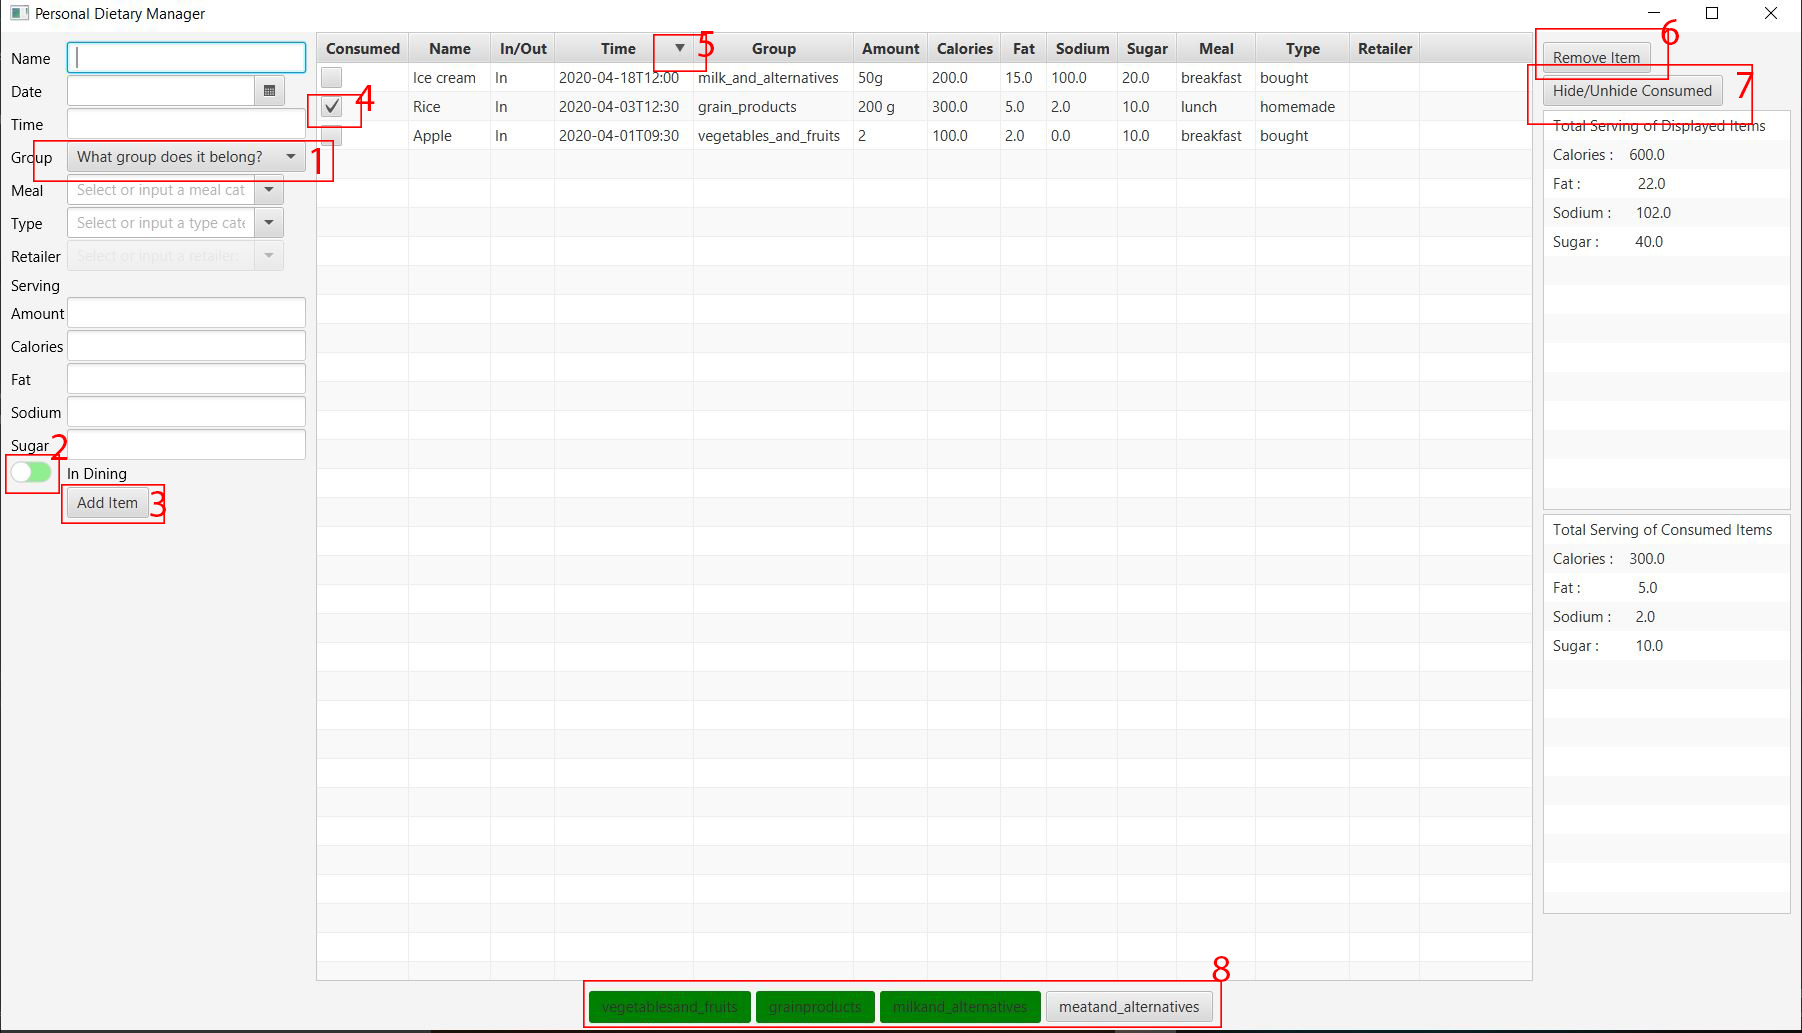
\includegraphics[scale=0.4]{Screenshot.jpg}

    \subsection{Image 1: Food group combo box}

	\newcolumntype{a}{>{\columncolor{pink}}c}	
	\def\arraystretch{1.5}
		\begin{tabular}{|a|p{13cm}|}
	\hline
		\textbf{Use Case} & 4.3.2 Add a food item \\
	\hline
		 \textbf{Description} & Drop down menu to select food group of added item \\ 
	\hline
		\textbf{Preconditions} &  Application is open; data has been properly entered \\
	\hline
		\textbf{Postconditions} & Food item appears with proper food group \\
	\hline
		\textbf{Comments} & Test sucessful \\
	\hline
	\end{tabular}

   \subsection{Image 2: Indining/outdining toggle switch}

	\newcolumntype{a}{>{\columncolor{pink}}c}	
	\def\arraystretch{1.5}
		\begin{tabular}{|a|p{13cm}|}
	\hline
		\textbf{Use Case} & 4.3.8 Choose a food item as either indining or outdining \\
	\hline
		 \textbf{Description} & Toggle between indining and outdining food attribute \\ 
	\hline
		\textbf{Preconditions} &  Application is open; data has been properly entered \\
	\hline
		\textbf{Postconditions} & Food item appears with proper indining or outdining attribute \\
	\hline
		\textbf{Comments} & Test sucessful \\
	\hline
	\end{tabular}

   \subsection{Image 3: Food add button}

	\newcolumntype{a}{>{\columncolor{pink}}c}	
	\def\arraystretch{1.5}
		\begin{tabular}{|a|p{13cm}|}
	\hline
		\textbf{Use Case} & 4.3.2 Add a food item \\
	\hline
		 \textbf{Description} & Add a food item \\ 
	\hline
		\textbf{Preconditions} &  Application is open; data has been properly entered \\
	\hline
		\textbf{Postconditions} & Food item appears with proper food attributes \\
	\hline
		\textbf{Comments} & Test sucessful \\
	\hline
	\end{tabular}

   \subsection{Image 4: Consumed checkbox}

	\newcolumntype{a}{>{\columncolor{pink}}c}	
	\def\arraystretch{1.5}
		\begin{tabular}{|a|p{13cm}|}
	\hline
		\textbf{Use Case} & 4.3.7 Set a food item as consumed or not consumed \\
	\hline
		 \textbf{Description} & Checkbox for setting food attribute as consumed or not consumed \\ 
	\hline
		\textbf{Preconditions} &  Food item is present in center list \\
	\hline
		\textbf{Postconditions} & Food item appears either as consumed, or not consumed; right-bottom serving box is updated \\
	\hline
		\textbf{Comments} & Test sucessful \\
	\hline
	\end{tabular}

   \subsection{Image 5: Table column button}

	\newcolumntype{a}{>{\columncolor{pink}}c}	
	\def\arraystretch{1.5}
		\begin{tabular}{|a|p{13cm}|}
	\hline
		\textbf{Use Case} & 4.3.6 Sort the food list based on a food attribute (e.g. serving, time, food group) \\
	\hline
		 \textbf{Description} & Button to sort (ascending or descending) list of food based on alphanumeric values \\ 
	\hline
		\textbf{Preconditions} &  Food items are present in center list \\
	\hline
		\textbf{Postconditions} & Food items appear sorted based on selected attribute \\
	\hline
		\textbf{Comments} & Test sucessful \\
	\hline
	\end{tabular}

   \subsection{Image 6: Remove button}

	\newcolumntype{a}{>{\columncolor{pink}}c}	
	\def\arraystretch{1.5}
		\begin{tabular}{|a|p{13cm}|}
	\hline
		\textbf{Use Case} & 4.3.5 Remove a food item \\
	\hline
		 \textbf{Description} & Removes the selected food item from the food list \\ 
	\hline
		\textbf{Preconditions} &  Food item(s) is present in center list; food item is selected \\
	\hline
		\textbf{Postconditions} &  Selected food item is removed from list \\
	\hline
		\textbf{Comments} & Test sucessful \\
	\hline
	\end{tabular}

   \subsection{Image 7: Hide/Unhide Consumed button}

	\newcolumntype{a}{>{\columncolor{pink}}c}	
	\def\arraystretch{1.5}
		\begin{tabular}{|a|p{13cm}|}
	\hline
		\textbf{Use Case} & 4.3.9 View only consumed food items, or view all food items \\
	\hline
		 \textbf{Description} & Shows list of either all food items, or only consumed food items \\ 
	\hline
		\textbf{Preconditions} &  Food items are present in center list; at least one food item is set to consumed \\
	\hline
		\textbf{Postconditions} &  Either list of all food items, or only consumed food items, is shown; top-right display is updated\\
	\hline
		\textbf{Comments} & Test sucessful \\
	\hline
	\end{tabular}

   \subsection{Image 8: Food group button}

	\newcolumntype{a}{>{\columncolor{pink}}c}	
	\def\arraystretch{1.5}
		\begin{tabular}{|a|p{13cm}|}
	\hline
		\textbf{Use Case} & 4.3.3 Mark a food group as eaten or not eaten \\
	\hline
		 \textbf{Description} & Lights up when a food is in the list with the given food attribute \\ 
	\hline
		\textbf{Preconditions} &  Food items are present in food list \\
	\hline
		\textbf{Postconditions} & Buttons at bottom are light up with relevant food groups\\
	\hline
		\textbf{Comments} & Test sucessful \\
	\hline
	\end{tabular}
    \chapter{Database UML Class Diagram}
    
    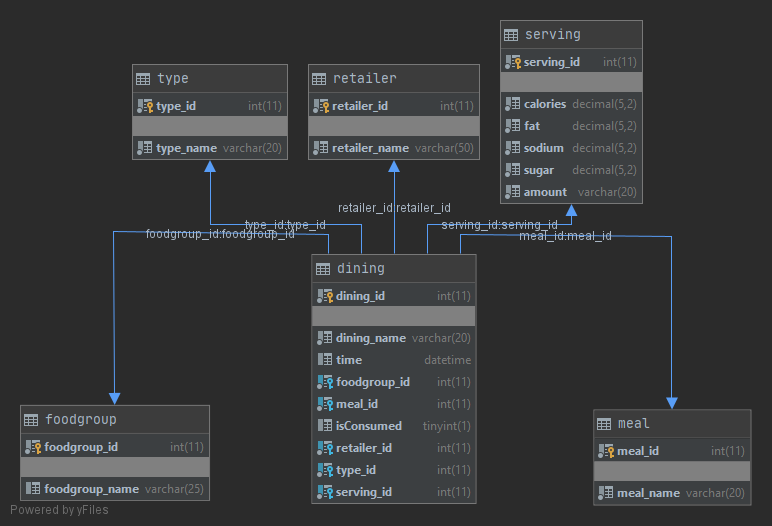
\includegraphics[scale=0.6]{db-uml.png}

\end{document}